\chapter{Benchmarks and Metrics in Industry}\label{ch:benchmarks_and_metrics}
In this chapter all the tools and the benchmarks for object localization and detection will be exposed. In particular, first the metrics and the techniques used to evaluate pose estimations will be presented, then some publicly available datasets will be presented. 

The problems that are going to be tackled are related to the 6D object pose estimation task. A 6D object pose is mathematically the 3D position of the object in the space plus 3 more terms that describe its rotation:

\begin{equation}
    \label{eq:6D_obj_pose_0}
    \hat{P} = (x, y, z, \alpha_x, \alpha_y, \alpha_z)^T
\end{equation}

The Eq. \ref{eq:6D_obj_pose_0} refers to the 6D pose estimate of an object, the first three terms $x, y, z$ describe the position in the camera reference frame, while the last three terms $\alpha_x, \alpha_y, \alpha_z$ represent the object's rotation angles along the $x, y, z$ camera axis respectively. This formulation can be easily manipulated in terms of rotation matrices and translation vectors:

\begin{equation}
    \label{eq:6D_obj_pose_1}
    \hat{P} = (R, t)
\end{equation}

The Eq. \ref{eq:6D_obj_pose_1} is a manipulated version of \ref{eq:6D_obj_pose_0} where the rotation matrix $R$ encodes the three angles of rotation $\alpha_x, \alpha_y, \alpha_z$ and the translation vector $t$ encodes the $x, y, z$ position of the object in the reference frame of the camera.

\begin{figure}
	\centering
	\begin{subfigure}{.5\textwidth}
  		\centering
  		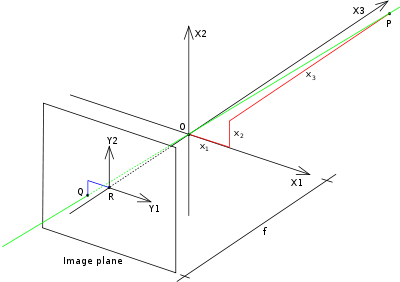
\includegraphics[width=.8\linewidth]{figures/2_benchmarks_and_metrics/pinhole_geometry_3D}
  		\caption{3D view}
  		\label{fig:sub1}
	\end{subfigure}%
	\begin{subfigure}{.5\textwidth}
  		\centering
  		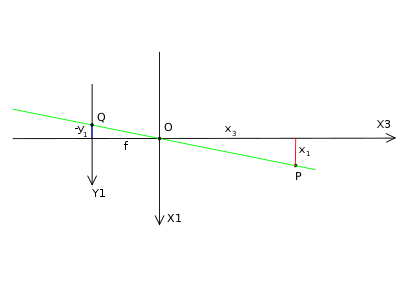
\includegraphics[width=.8\linewidth]{figures/2_benchmarks_and_metrics/pinhole_geometry_2D}
  		\caption{2D view}
  		\label{fig:sub2}
	\end{subfigure}
	\caption{\textbf{Pinhole Camera Geometry.} In (A) the geometry of the pinhole camera in 3D view, in (B) its 2D representation.}
	\label{fig:test}
\end{figure}

Each object pose estimate can also be projected back to the camera image plane. This projection between the 3D space and the 2D space of the image plane is achieved by applying the projection obtained with a given camera matrix model. The camera model that we consider here is the so called Pinhole Camera Model, and it's geometry is depicted in Figure 

Given this first formulation for the 6D pose of an object, and its relative pose within the image plane, we can now address the problem of defining how good is a pose estimate.

\section{Metrics}\label{sec:metrics}


\section{Industrially oriented Datasets}\label{sec:datasets}
To do ...

\subsection{T-LESS Dataset}\label{subsec:tless_dataset}
To do ...

\subsection{MVTec ITODD}\label{subsec:mvtex_itodd}
To do ...